\section{Radio Operating Essentials}
\label{section:operating_essentials}

\subsection*{Band Plans}
A band plan is a voluntary guideline for using different modes or activities within an amateur radio band. It helps operators organize their use of the frequency spectrum, ensuring that various types of communications (such as voice, digital, and Morse code) can coexist without interference. Band plans are not enforced by the FCC but are widely adopted by the amateur radio community to promote efficient and harmonious use of the available frequencies.

\subsection*{Simplex vs. Duplex Communication}
Simplex communication refers to a mode where transmission and reception occur on the same frequency. This is commonly used for direct communication between two stations without the need for a repeater. For example, two operators might communicate directly on 146.520 MHz (the national 2-meter FM simplex calling frequency).

Duplex communication involves transmitting and receiving on two different frequencies, often facilitated by a repeater. When using a repeater, your radio transmits on one frequency (the repeater's input) and receives on another frequency (the repeater's output). This allows for simultaneous two-way communication, which is particularly useful in scenarios where direct communication is not feasible due to distance or obstacles.

Semi-duplex operation, a common form of duplex communication in amateur radio, occurs when stations take turns transmitting and receiving on different frequencies. This is the typical mode when using repeaters - while one station transmits, others listen on the repeater's output frequency.

\begin{figure}[h]
    \centering
    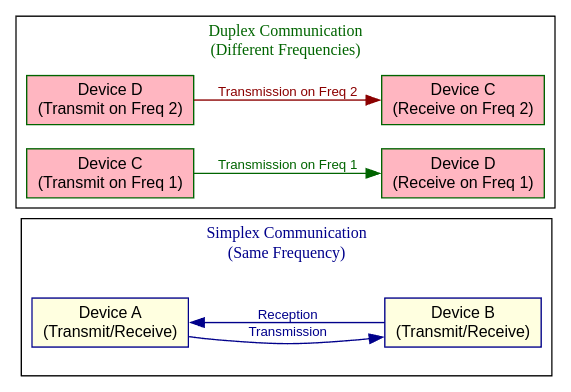
\includegraphics[width=0.8\textwidth]{tech/organized/chapter_2/images/simplex_duplex_diagram.png}
    \caption{Simplex vs. Duplex Communication}
    \label{fig:simplex_duplex}
    % Diagram illustrating the difference between simplex and duplex communication.
    % The diagram should show two scenarios: one where both transmission and reception occur on the same frequency (simplex), and another where transmission and reception occur on different frequencies (duplex).
\end{figure}


\subsection*{CTCSS and DTMF Tones}
CTCSS (Continuous Tone-Coded Squelch System) and DTMF (Dual-Tone Multi-Frequency) are two different tone systems used in amateur radio, each serving distinct purposes.

\textbf{CTCSS} tones, also known as PL (Private Line) tones, are sub-audible tones (below 300 Hz) that are transmitted along with your voice. These tones act as a "key" to open the squelch of a receiver. When enabled:
\begin{itemize}
    \item The tone is continuously transmitted with your voice
    \item Receivers only open their squelch when detecting the correct tone
    \item Helps reduce interference from other stations
    \item Commonly used for repeater access control
\end{itemize}

\begin{table}[h]
    \centering
    \caption{Standard CTCSS Frequencies and Common Names}
    \begin{tabular}{|l|l||l|l||l|l||l|l|}
        \hline
        \textbf{Hz} & \textbf{Code} & \textbf{Hz} & \textbf{Code} & \textbf{Hz} & \textbf{Code} & \textbf{Hz} & \textbf{Code} \\
        \hline
        67.0 & XZ & 91.5 & ZZ & 118.8 & 2B & 156.7 & 5A \\
        71.9 & XA & 94.8 & ZA & 123.0 & 3Z & 162.2 & 5B \\
        74.4 & WA & 97.4 & ZB & 127.3 & 3A & 167.9 & 6Z \\
        77.0 & XB & 100.0 & 1Z & 131.8 & 3B & 173.8 & 6A \\
        79.7 & SP & 103.5 & 1A & 136.5 & 4Z & 179.9 & 6B \\
        82.5 & YZ & 107.2 & 1B & 141.3 & 4A & 186.2 & 7Z \\
        85.4 & YA & 110.9 & 2Z & 146.2 & 4B & 192.8 & 7A \\
        88.5 & YB & 114.8 & 2A & 151.4 & 5Z & 203.5 & M1 \\
        \hline
    \end{tabular}
    \label{tab:ctcss_tones}
\end{table}

These CTCSS codes are often referred to as "PL tones" (Private Line, a Motorola trademark) or "sub-audible tones." The code designations (like "XZ", "1A", etc.) are standard references used by manufacturers and repeater coordinators. For example, if a repeater requires "PL 103.5" or "tone 1A", both refer to the same 103.5 Hz CTCSS tone.

\textbf{DTMF} tones, commonly known as "Touch-Tones," are pairs of audible frequencies used for sending commands or control signals. Each digit or symbol combines one tone from a low frequency group with one from a high frequency group. When you press a button on your radio's keypad:
\begin{itemize}
    \item Two tones are generated simultaneously
    \item One tone comes from the row frequency (697-941 Hz)
    \item One tone comes from the column frequency (1209-1633 Hz)
    \item The combination uniquely identifies each key
\end{itemize}

For example:
\begin{itemize}
    \item Pressing "5" generates 770 Hz (row) + 1336 Hz (column)
    \item Pressing "9" generates 852 Hz (row) + 1477 Hz (column)
    \item The "*" key generates 941 Hz + 1209 Hz
\end{itemize}

DTMF is used for:
\begin{itemize}
    \item Remote control of repeaters
    \item Autopatch systems (connecting to telephone lines)
    \item Accessing repeater features
    \item Other control functions
\end{itemize}

\begin{table}[h]
    \centering
    \caption{DTMF Tone Pairs (Hz)}
    \begin{tabular}{|c||c|c|c|c|}
        \hline
        & 1209 Hz & 1336 Hz & 1477 Hz & 1633 Hz \\
        \hline
        697 Hz & 1 & 2 & 3 & A \\
        \hline
        770 Hz & 4 & 5 & 6 & B \\
        \hline
        852 Hz & 7 & 8 & 9 & C \\
        \hline
        941 Hz & * & 0 & \# & D \\
        \hline
    \end{tabular}
    \label{tab:dtmf_tones}
\end{table}

Unlike CTCSS tones, DTMF tones are meant to be heard and are only transmitted when you press the corresponding buttons. This system is the same technology that traditional touch-tone phones use, which is why it's compatible with telephone systems when using autopatch features.

\subsection*{Linked Repeater Networks}
A linked repeater network is a system where multiple repeaters are interconnected, allowing signals received by one repeater to be transmitted by all the repeaters in the network. This extends the range of communication and enables operators to communicate over much larger areas than would be possible with a single repeater. Linked repeater networks are particularly useful in emergency situations where wide-area communication is essential.

\subsection*{Questions}
\begin{tcolorbox}[colback=gray!10!white,colframe=black!75!black,title={T2A09}]
    Which of the following indicates that a station is listening on a repeater and looking for a contact?
    \begin{enumerate}[label=\Alph*),noitemsep]
        \item “CQ CQ” followed by the repeater’s call sign
        \item \textbf{The station’s call sign followed by the word “monitoring”}
        \item The repeater call sign followed by the station’s call sign
        \item “QSY” followed by your call sign
    \end{enumerate}
\end{tcolorbox}
When a station is monitoring a repeater and looking for a contact, it typically identifies itself by its call sign followed by the word "monitoring." This indicates that the station is listening and available for communication.

%memory_trick T2A09

\begin{tcolorbox}[colback=gray!10!white,colframe=black!75!black,title={T2A10}]
    What is a band plan, beyond the privileges established by the FCC?
    \begin{enumerate}[label=\Alph*),noitemsep]
        \item \textbf{A voluntary guideline for using different modes or activities within an amateur band}
        \item A list of operating schedules
        \item A list of available net frequencies
        \item A plan devised by a club to indicate frequency band usage
    \end{enumerate}
\end{tcolorbox}
A band plan is a voluntary guideline that helps amateur radio operators organize their use of the frequency spectrum. It is not enforced by the FCC but is widely adopted to ensure efficient and harmonious use of the available frequencies.

%memory_trick T2A10

\begin{tcolorbox}[colback=gray!10!white,colframe=black!75!black,title={T2A11}]
    What term describes an amateur station that is transmitting and receiving on the same frequency?
    \begin{enumerate}[label=\Alph*),noitemsep]
        \item Full duplex
        \item Diplex
        \item \textbf{Simplex}
        \item Multiplex
    \end{enumerate}
\end{tcolorbox}
Simplex communication involves transmitting and receiving on the same frequency. This is commonly used for direct communication between two stations without the need for a repeater.

%memory_trick T2A11

\begin{tcolorbox}[colback=gray!10!white,colframe=black!75!black,title={T2A12}]
    What should you do before calling CQ?
    \begin{enumerate}[label=\Alph*),noitemsep]
        \item Listen first to be sure that no one else is using the frequency
        \item Ask if the frequency is in use
        \item Make sure you are authorized to use that frequency
        \item \textbf{All these choices are correct}
    \end{enumerate}
\end{tcolorbox}
Before calling CQ, it is important to listen to ensure the frequency is not in use, ask if the frequency is in use, and confirm that you are authorized to use that frequency. All these steps are essential to avoid interference and ensure proper operation.

%memory_trick T2A12

\begin{tcolorbox}[colback=gray!10!white,colframe=black!75!black,title={T2B01}]
    How is a VHF/UHF transceiver’s “reverse” function used?
    \begin{enumerate}[label=\Alph*),noitemsep]
        \item To reduce power output
        \item To increase power output
        \item \textbf{To listen on a repeater’s input frequency}
        \item To listen on a repeater’s output frequency
    \end{enumerate}
\end{tcolorbox}
The "reverse" function on a VHF/UHF transceiver is used to listen on a repeater's input frequency. This allows the operator to hear what is being transmitted directly to the repeater, which can be useful for troubleshooting or monitoring.

%memory_trick T2B01

\begin{tcolorbox}[colback=gray!10!white,colframe=black!75!black,title={T2B02}]
    What term describes the use of a sub-audible tone transmitted along with normal voice audio to open the squelch of a receiver?
    \begin{enumerate}[label=\Alph*),noitemsep]
        \item Carrier squelch
        \item Tone burst
        \item DTMF
        \item \textbf{CTCSS}
    \end{enumerate}
\end{tcolorbox}
CTCSS (Continuous Tone-Coded Squelch System) uses a sub-audible tone transmitted along with normal voice audio to open the squelch of a receiver. This ensures that only signals with the correct tone are heard, reducing interference from other transmissions.

%memory_trick T2B02

\begin{tcolorbox}[colback=gray!10!white,colframe=black!75!black,title={T2B03}]
    Which of the following describes a linked repeater network?
    \begin{enumerate}[label=\Alph*),noitemsep]
        \item \textbf{A network of repeaters in which signals received by one repeater are transmitted by all the repeaters in the network}
        \item A single repeater with more than one receiver
        \item Multiple repeaters with the same control operator
        \item A system of repeaters linked by APRS
    \end{enumerate}
\end{tcolorbox}
A linked repeater network is a system where multiple repeaters are interconnected, allowing signals received by one repeater to be transmitted by all the repeaters in the network. This extends the range of communication and is particularly useful in emergency situations.

%memory_trick T2B03

\begin{tcolorbox}[colback=gray!10!white,colframe=black!75!black,title={T2B04}]
    Which of the following could be the reason you are unable to access a repeater whose output you can hear?
    \begin{enumerate}[label=\Alph*),noitemsep]
        \item Improper transceiver offset
        \item You are using the wrong CTCSS tone
        \item You are using the wrong DCS code
        \item \textbf{All these choices are correct}
    \end{enumerate}
\end{tcolorbox}
If you can hear a repeater's output but cannot access it, the issue could be due to an improper transceiver offset, using the wrong CTCSS tone, or using the wrong DCS code. All these factors can prevent successful communication with the repeater.

%memory_trick T2B04

\subsection*{Summary}
\begin{itemize}
    \item \textbf{Band Plans}: Voluntary guidelines for organizing the use of different modes and activities within amateur radio bands.
    \item \textbf{Simplex vs. Duplex}: Simplex involves transmitting and receiving on the same frequency, while duplex uses separate frequencies for transmission and reception.
    \item \textbf{CTCSS and DTMF Tones}: Used in repeater operations to control access and improve communication quality.
    \item \textbf{Linked Repeater Networks}: Systems where multiple repeaters are interconnected to extend communication range and improve reliability.
\end{itemize}
